\section{Merkle-DAG Architecture}

\label{sec:merkle}

\subsection{Design Goals}

The Experience Ledger data structure must support:

\begin{enumerate}
    \item $O(\log n)$ membership verification
    \item $O(1)$ content retrieval by CID
    \item $O(\log n)$ approximate nearest neighbor search
    \item Efficient incremental updates
    \item Verifiable cross-library queries
\end{enumerate}

\subsection{Hybrid Merkle-DAG}

We propose a hybrid structure combining Merkle trees (for verification) with semantic DAGs (for retrieval):

\begin{figure}[t]
\centering
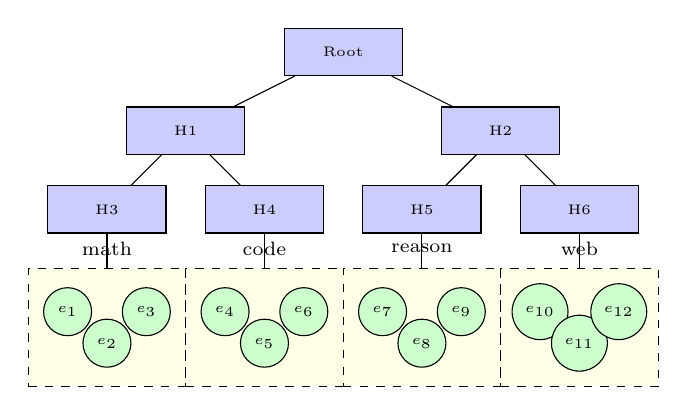
\begin{tikzpicture}[
    node distance=1cm,
    hash/.style={rectangle, draw, minimum width=1.5cm, minimum height=0.6cm, fill=blue!20, font=\tiny},
    exp/.style={circle, draw, minimum size=0.5cm, fill=green!20, font=\tiny},
    cluster/.style={rectangle, draw, dashed, minimum width=2cm, minimum height=1.5cm, fill=yellow!10}
]
    % Root
    \node[hash] (root) at (4,4) {Root};

    % Level 1
    \node[hash] (l1a) at (2,3) {H1};
    \node[hash] (l1b) at (6,3) {H2};

    % Level 2
    \node[hash] (l2a) at (1,2) {H3};
    \node[hash] (l2b) at (3,2) {H4};
    \node[hash] (l2c) at (5,2) {H5};
    \node[hash] (l2d) at (7,2) {H6};

    % Clusters (semantic)
    \node[cluster] (c1) at (1,0.5) {};
    \node[cluster] (c2) at (3,0.5) {};
    \node[cluster] (c3) at (5,0.5) {};
    \node[cluster] (c4) at (7,0.5) {};

    % Experiences in clusters
    \node[exp] at (0.5,0.7) {$e_1$};
    \node[exp] at (1,0.3) {$e_2$};
    \node[exp] at (1.5,0.7) {$e_3$};

    \node[exp] at (2.5,0.7) {$e_4$};
    \node[exp] at (3,0.3) {$e_5$};
    \node[exp] at (3.5,0.7) {$e_6$};

    \node[exp] at (4.5,0.7) {$e_7$};
    \node[exp] at (5,0.3) {$e_8$};
    \node[exp] at (5.5,0.7) {$e_9$};

    \node[exp] at (6.5,0.7) {$e_{10}$};
    \node[exp] at (7,0.3) {$e_{11}$};
    \node[exp] at (7.5,0.7) {$e_{12}$};

    % Edges
    \draw[-] (root) -- (l1a);
    \draw[-] (root) -- (l1b);
    \draw[-] (l1a) -- (l2a);
    \draw[-] (l1a) -- (l2b);
    \draw[-] (l1b) -- (l2c);
    \draw[-] (l1b) -- (l2d);
    \draw[-] (l2a) -- (c1);
    \draw[-] (l2b) -- (c2);
    \draw[-] (l2c) -- (c3);
    \draw[-] (l2d) -- (c4);

    % Labels
    \node[font=\scriptsize] at (1,1.5) {math};
    \node[font=\scriptsize] at (3,1.5) {code};
    \node[font=\scriptsize] at (5,1.5) {reason};
    \node[font=\scriptsize] at (7,1.5) {web};
\end{tikzpicture}
\caption{Hybrid Merkle-DAG structure: Merkle tree for verification (blue), semantic clusters for retrieval (yellow), individual experiences (green).}
\label{fig:merkle-dag}
\end{figure}

\subsection{Semantic Clustering}

Experiences are grouped into clusters based on embedding similarity:

\begin{algorithm}[t]
\caption{Semantic Cluster Construction}
\label{alg:cluster}
\begin{algorithmic}[1]
\STATE \textbf{Input}: Experience set $\mathcal{E}$, cluster count $k$
\STATE \textbf{Output}: Clusters $\{C_1, \ldots, C_k\}$, centroids $\{\mu_1, \ldots, \mu_k\}$
\STATE $\{\mu_i\} \leftarrow \text{k-means++}(\{e.v \mid e \in \mathcal{E}\}, k)$
\FOR{$e \in \mathcal{E}$}
    \STATE $i^* \leftarrow \arg\min_i \|e.v - \mu_i\|_2$
    \STATE $C_{i^*} \leftarrow C_{i^*} \cup \{e\}$
\ENDFOR
\RETURN $\{C_i\}, \{\mu_i\}$
\end{algorithmic}
\end{algorithm}

\subsection{Merkle Tree Construction}

Each cluster is hashed into a Merkle leaf, then aggregated:

\begin{equation}
H_{\text{cluster}}(C_i) = \text{SHA256}\left(\bigoplus_{e \in C_i} \text{CID}(e)\right)
\end{equation}

where $\bigoplus$ denotes sorted concatenation.

\begin{equation}
H_{\text{parent}}(H_1, H_2) = \text{SHA256}(H_1 \| H_2)
\end{equation}

The root hash $r$ commits to the entire library:

\begin{equation}
r = \text{MerkleRoot}(\{H_{\text{cluster}}(C_i)\}_{i=1}^k)
\end{equation}

\subsection{Proof Structure}

A Merkle proof $\pi$ for experience $e$ consists of:

\begin{equation}
\pi = (e, i, \{h_j, \text{side}_j\}_{j=1}^{\lceil \log_2 k \rceil})
\end{equation}

where $h_j$ are sibling hashes and $\text{side}_j \in \{\text{L}, \text{R}\}$ indicates position.

\begin{theorem}[Proof Verification]
Given root $r$, experience $e$, and proof $\pi$, verification succeeds iff:
\begin{equation}
\text{VerifyProof}(r, e, \pi) = \mathbb{1}[\text{ReconstructRoot}(\text{CID}(e), \pi) = r]
\end{equation}
\end{theorem}

